\documentclass{article}
\usepackage{amsmath}
\usepackage{mathtools}
\usepackage{gensymb}
\usepackage[a4paper,inner=1.5cm,outer=1.5cm,top=2cm,bottom=0.5cm]{geometry} 
\usepackage{xcolor}                    
\usepackage{tikz}                           
\usepackage{multicol}
\usepackage{pgfplots}
\usetikzlibrary{calc}
\usetikzlibrary{intersections}
\usetikzlibrary{intersections,calc,angles,quotes}
\usetikzlibrary{shapes,arrows,positioning,decorations.pathreplacing,calc}
\usetikzlibrary{calc,angles,positioning,intersections,quotes,decorations.markings}
\usepackage{tkz-euclide}
\usetikzlibrary{backgrounds}
\usetikzlibrary{calc,through}
\usetikzlibrary{angles}
\usetikzlibrary{fadings}
\usetikzlibrary{shapes.geometric}
\usetikzlibrary{shapes.symbols}
\usepackage{draftwatermark}
\usepackage{mathptmx}

\SetWatermarkText{\textcolor{black!30}{Mathema Shukur}}
\SetWatermarkFontSize{2 cm}
\usepackage[utf8]{inputenc}
\usepackage{fontspec}

\setmainfont{[Kalpurush.ttf]}
\newfontface{\en}{[Arial.ttf]} %%this is optional, if you want to use a secondary font. Any english font is supported
\newlength\Radius
\setlength\Radius{4cm}
\begin{document} 
	\Large
	\textcolor{red}{Welcome To} 
	\\
	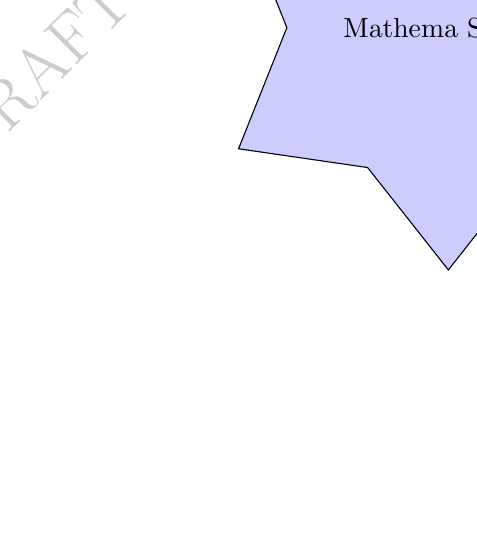
\begin{tikzpicture}
		\tikz \node [fill=blue!20,star,star points=6,draw] {Mathema Shukur };
	\end{tikzpicture}
	\\
	যাদের জন্যে প্রযোজ্যঃ  	\textcolor{magenta}{একাদশ ও দ্বাদশ শ্রেণীর শিক্ষার্থী} \\
	বিষয়ঃ \textcolor{magenta}{উচ্চতর গণিত ১ম পত্র} \\
	অধ্যায়ঃ \textcolor{magenta}{৩-সরলরেখা}\\ 
	Subtopicঃ  \textcolor{magenta}{  সরলরেখার বিভিন্ন আকারের সমীকরণ নির্ণয় করা   }\\
	\\
	\textcolor{blue}{(1)	ঢাল বিন্দু আকার Point slope form}\\
	\\
	$(y-y_1)=m(x-x_1)$\\
	\\
	\textcolor{red} {(2)  দুই বিন্দু আকার 	Two point form}\\
	\\
	$y-y_1=\left(\frac{y_1-y_2}{x_1-x_2}\right)(x-x_1)$\\
	\\
	\textcolor{green}{ (3) ঢাল খণ্ডন আকার 	Slope intercept form}\\
	\\
	$y=mx+c$\\
	\\
	\textcolor{cyan}{ (4) দ্বি খণ্ডন আকার  Two	Intercept form}\\
	\\
	$\frac{x}{a}+\frac{y}{b}=1$\\
	\\
\vspace{6cm}
\\
\textcolor{red} {(2)  দুই বিন্দু আকার 	Two point form}\\
\\
$y-y_1=\left(\frac{y_1-y_2}{x_1-x_2}\right)(x-x_1)$\\
\\
	কুমিল্লা বোর্ড-২০২১\\
	$(1,2)$ এবং  $(3,-2)$ বিন্দুগামী  সরলরেখার সমীকরণ নির্ণয় কর \\
	$(x_1,y_1)=(1,2)$\qquad $(x_2,y_2)=(3,-2)$\\ 
	\begin{align*}
y-y_1&=\left(\frac{y_1-y_2}{x_1-x_2}\right)(x-x_1)\\
y-2&=\left(\frac{2-(-2)}{1-3}\right)(x-1)\\
y-2&=\left(\frac{4}{-2}\right)(x-1)\\
		y-2&=-2(x-1)\\
		y-2&=-2x+2\\
		\\
		2x+y-4&=0	
	\end{align*}
	\\
		\begin{tikzpicture}[transform shape,scale=1]
		\draw [-latex,thick](-5,0) -- (5,0) node[right] {$x$} coordinate(x axis);
		\draw [-latex,thick](0,-5) -- (0,7) node[above] {$y$} coordinate(y axis);
		\fill[black] (0,0) circle (1 mm);
			\fill[magenta] (1,2) circle (1 mm);
				\fill[magenta] (3,-2) circle (1 mm);
		\node at (0.3,-0.3) {$\textcolor{purple}{O}$};	
			\node at (1.7,2) {$\textcolor{magenta}{(1,2)}$};	
				\node at (4,-2) {$\textcolor{magenta}{(3,-2)}$};	
		\draw[very thick,magenta] (-1,6)--(4,-4);	
	\end{tikzpicture}
\end{document}